\subsection{Standard Model W$\gamma$ Production}
\label{WgAbout_SMproduction}



%Your chapter 2.1 seems to be a collection of very different pieces. You define here what is a cross section, and discuss the golden rule, and talk about Largantian pieces, and talk about branching ratio values, and talk about experimental issues like detection efficiency and acceptance. In my opinion, this just doesn’t belong to the same 2-page paragraph. Consider sorting this with an appropriate structure of sections, expanding at more length if necessary.

%Check your logic. The sequence is odd. First you define what is a differential cross section, then later you define what "cross section" means at all.

%Consider discussing parton luminosity and the cross section expression that involves the PDFs and parton-based cross sections

%It feels in general that pieces are thrown in without justification or good transitions.
%For example, the Golden Rule comes from nowhere, without explanation of what it means or where it comes from (you just say that “one has to use” it).

%At places, you still have a choppy flow of sentences.

%There is a number of stylistic, word usage, formatting issues, but would rather leave it
%for later when you reshuffle the content a bit. To mention a few things:
%   - Write “Figure X” in full when in the beginning of the sentence, Fig. X when in the middle
%         (read again CMS Pubs Committee recommendations, it is there).
%   - write in math mode (bar over q)^prime and not bar over (q^prime)
%   - define “NNLO"


A $W$ boson in proton-proton collisions can be produced in the processes $q {\bar{q'}} \rightarrow W$ where $q$ and $\bar{q'}$ are a quark and an antiquark which have a total charge of $+1$ if producing a $W^+$ boson or of $-1$ if producing a $W^-$ boson. The processes $u\bar{d}\rightarrow W^+$ and $d\bar{u}\rightarrow W^-$ are the most likely to occur because $u$ and $d$ are valence quarks in a proton. Antiquarks $\bar{d}$ and $\bar{u}$ come from sea $q\bar{q}$ pairs of the other proton.\\

A $W$ boson decays immediately after being created, and we do not detect the $W$ boson itself but its decay products. Decay modes of a $W$ boson include $W^\pm \rightarrow l^\pm \nu_l ({\bar{\nu_l}})$ where $l^\pm=e^\pm$, $\mu^\pm$ or $\tau^\pm$ with branching fractions of ~11\% per a leptonic channel \cite{ref_PDG}. The rest 67\% stands for various $W\rightarrow q\bar{q'}$ decays. In this dissertation we only consider $W^\pm \rightarrow \mu^\pm \nu_\mu ({\bar{\nu_\mu}})$ and $W^\pm \rightarrow e^\pm \nu_e ({\bar{\nu_e}})$ as the cleanest channels.\\

% MAY NOT NEED THIS
%Mass of a $W$ boson $M_W=80$ GeV is much larger than masses of its decay products: $M_\mu=105$ MeV, $M_e=0.5$ MeV, $M_\nu<2$ eV. Therefore, almost all mass of a $W$ boson converts to the kinetic energy of the muon or electron and neutrino or antineutrino.\\

A photon can be emitted from any charged particle of the process: a quark, an antiquark, a charged lepton or a $W$ boson (Fig. \ref{fig:feynmWg_LO_NLO}, top). A quark and an antiquark are initial state particles and, therefore, if one of them radiates a photon, we call such process the Initial State Radiation (ISR). A muon or an electron is a final state particle and if it radiates a photon, we call such process the Final State Radiation (FSR). Finally, a $W$ boson is a gauge boson and if it radiates a photon, the process has a vertex with three gauge bosons: $WW\gamma$, and we call such process the Triple Gauge Coupling (TGC).\\

\begin{figure}[htb]
  \begin{center}
    {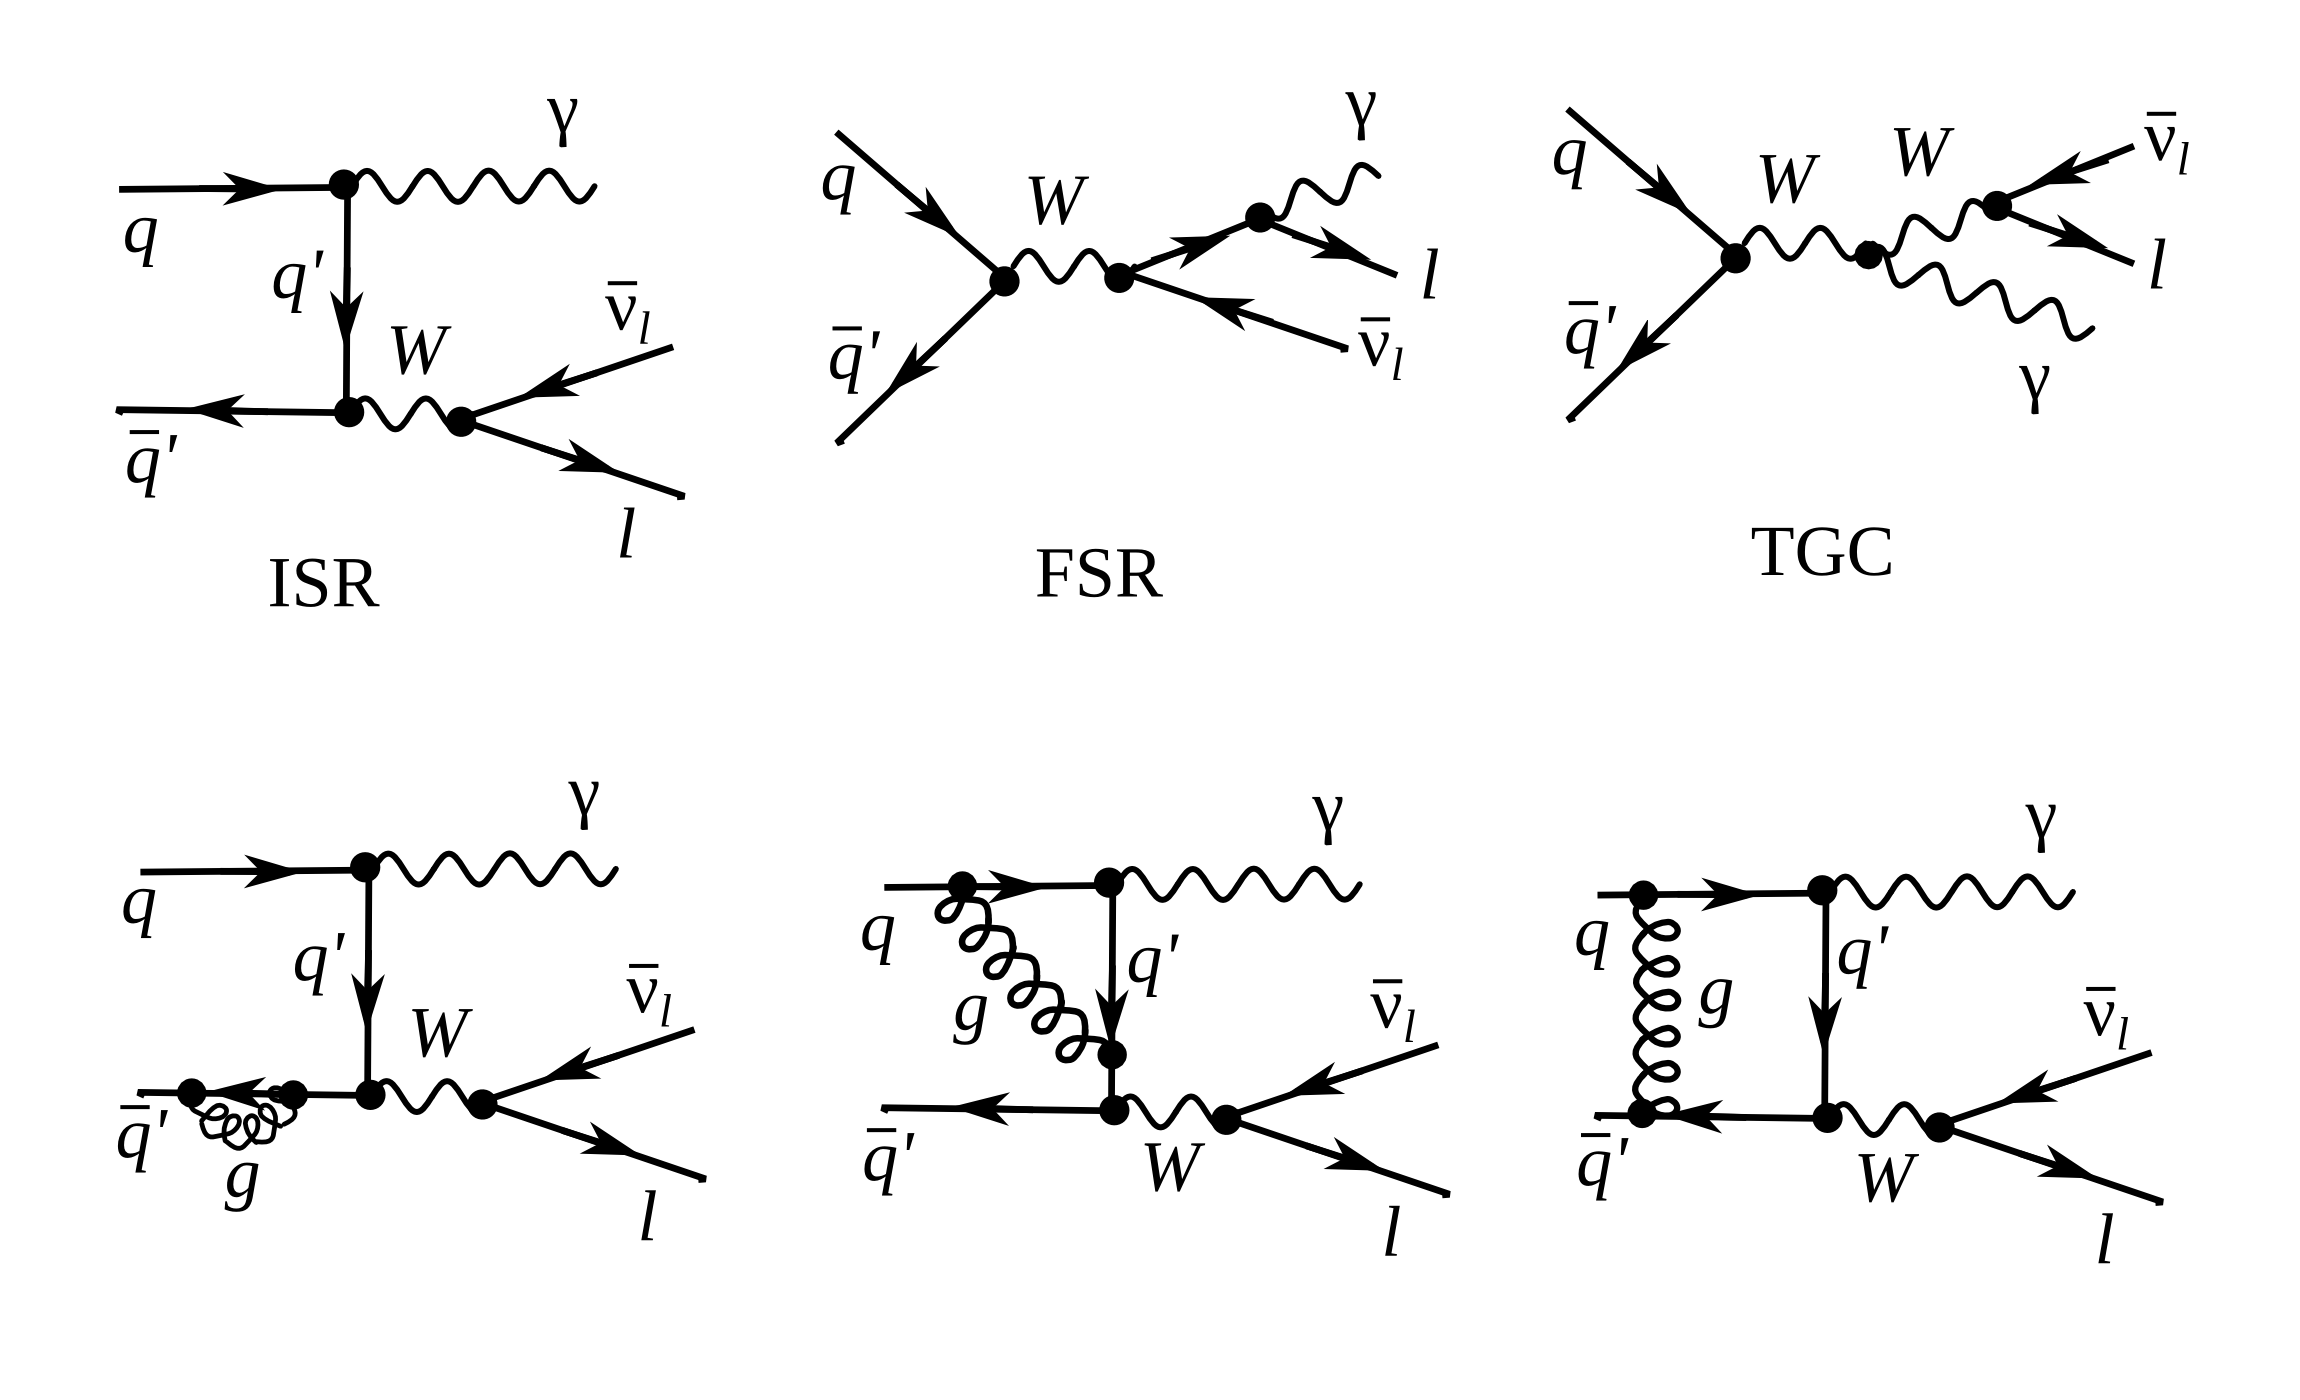
\includegraphics[width=0.90\textwidth]{../figs/WgAbout/feynmWg_LO_NLO.png}}
    \caption{Feynman diagrams of W$\gamma$ production}
    \label{fig:feynmWg_LO_NLO}
  \end{center}
\end{figure}

To represent the process graphically Feynman diagrams were invented. Also the diagrams can be used to calculate the process amplitude because they are determined by Lagrangian terms relevant to the process.\\

The electroweak Lagrangian is described in Chapter~\ref{sec:WgAbout_SMEWK}. It is possible to derive equations of motion from the Lagrangian for any fields involved \cite{ref_Griffiths}. However they cannot be solved exactly and, therefore, the perturbative approach is used if coupling constants are $g \ll 1$.\\

There is infinite number of Feynman diagrams corresponding to any specific process and the total amplitude of the process is a sum of individual amplitudes of each diagram and it is not technically possible to take into account all of them. The perturbative approach arranges all the diagrams by orders of contribution because each vertex is assigned a coupling constant and, therefore, the Feynman diagrams with fewer vertices would give a significantly larger contribution to the amplitude. In Fig. \ref{fig:feynmWg_LO_NLO} we have examples of the Leading Order (LO) and the Next-to-Leading Order (NLO) Feynman diagrams (top and bottom diagrams respectively).\\

The NLO corrections shown in Fig. \ref{fig:feynmWg_LO_NLO} are QCD corrections only which include gluon loops at the same quark line and exchange of a gluon between two different quark lines hovewer QED and weak NLO diagrams are also possible. QED corrections mean radiations of extra photons by charged particles, exchange of photons between different charged particles or a photon can be radiated and absorbed by the same charged particle forming a loop. Similarly, weak corrections mean extra virtual $W$ or $Z$ bosons. But the QCD corrections are the largest.\\

The theoretical cross section in particle physics is important not only for analysing the measurement result but also for producing the simulation which is then actively used while performing the measurement. The simulation consists of two parts: the generation of the process and the simulation of the particles paths through the detector. While the second one depends on the well-known properties of the particles and the detector configurations, the first part relies on the theory.\\

The most precise theoretical $W\gamma$ cross section available is the Next-to-Next-to-Leading Order (NNLO) cross section in QCD \cite{ref_theory_NNLO}. The effect of the NNLO correction ranges from 19\% to 26\% compared to the NLO cross section depending on the selection conditions. The contributions from the higher order corrections is estimated to be $\pm$4\%. However, the NNLO theoretical result was published in 2015 only and there is still no simulation available based on that result. The simulation used in this analisys is LO + up to two hadronic jets simulation which found to give the same predictions as the NLO result [REFERENCE to APPENDIX?].\\

In addition to the SM predictions, there are certain BSM theories which predict an enchancement of the contribution from the TGC diagram. The discussion of these BSM effects on the $W\gamma$ process takes place in chapter \ref{sec:WgAbout_ATGC}.\\ 


